\documentclass[11pt]{article}
\usepackage{graphicx}
\usepackage{lscape}
\usepackage{pdfpages}
\usepackage{scrextend}
\usepackage{gensymb}
\usepackage{subcaption}
\usepackage{rotating}
\usepackage[titletoc]{appendix}
\usepackage{setspace}
\usepackage{caption, float, multirow}

\setlength{\oddsidemargin}{0.3in}
\setlength{\textwidth}{5.9in}
\setlength{\topmargin}{-0.4in}
\setlength{\textheight}{8.5in}

\makeatletter
    \setlength\@fptop{0\p@}
\makeatother

\begin{document}

\doublespacing

\title{\textbf{Applicability of the Composite Rule-of-Mixtures for the Description of the Mechanical Properties of PBT Polymeric Matrix-Short Glass Fiber System}}
\author{Jan Quijalvo, Ryan Lam, Alan Wu}
\date{\today}


\makeatletter
    \singlespacing
    \begin{titlepage}
        \begin{center}
        	\begin{figure}[h]
        	\centering
            \includegraphics[scale=0.3]{./figures/University-of-Waterloo}
            \end{figure}
            \vspace{20mm}
            {\huge \bfseries  \@title }\\[2ex] 
            \vspace{5mm}
            {\LARGE Jan Quijalvo (20456787)}\\
            \vspace{2mm}
            {\LARGE Ryan Lam}\\
            \vspace{2mm}
            {\LARGE Alan Wu}\\
            \vspace{2mm}
            \LARGE 4B Mechanical Engineering\\[12ex]
            Prepared for\\
            ME 533 - Non-Metallic and Composite Materials\\
            Robert A. Varin
            \centering
            \vfill
            {\large April 3, 2017}
        \end{center}
    \end{titlepage}
\makeatother

\tableofcontents
\newpage
\listoffigures
\newpage
\listoftables
\newpage

\section{Introduction}
This lab is meant to demonstrate the applicability of the composite rule of mixtures to describe the mechanical properties of PBT polymeric matrix, short glass fiber systems. Most importantly is to look at its applicability to the material properties of Young's Modulus and fracture strength. PBT is an abbreviation for Polybutylene Terephthalate, a semi-crystalline thermoplastic engineering plastic widely used as a matrix for glass reinforced composites \cite{pbt}. PBT is a widely used plastic as a result of many desirable properties including high dimensional stability, high hardness, stiffness, chemical resistance, and processability. Some common uses for PBT include injection molded parts, electrical parts enclosures, and automotive trim \cite{pbt}. Important mechanical properties necessary for composite property calculations include:

\begin{table}[htb!]
\caption{Some important mechanical properties for PBT \cite{PBTmechProperties}.}
\label{mechProperties}
\begin{center}
\begin{tabular}{ p{6cm} || p{2cm}}
\textit{\textbf{Property}}& \textit{\textbf{Value}}\\
\hline

Young's Modulus [GPa] &  
\begin{minipage}[t]{1\textwidth}
	1.93 - 3
\end{minipage}\\

Shear Modulus [GPa] &  
\begin{minipage}[t]{1\textwidth}
	0.6902 - 1.073
\end{minipage}\\

Yield Strength [MPa] &  
\begin{minipage}[t]{1\textwidth}
	50 - 60
\end{minipage}\\ 

\% Elongation [\%] &  
\begin{minipage}[t]{1\textwidth}
	0.5 - 3
\end{minipage}\\ 

Density [g/\(cm^3\)] &  
\begin{minipage}[t]{1\textwidth}
	1.3 - 1.38
\end{minipage}\\ 

\end{tabular}
\end{center}
\end{table}

The reinforcement, commonly refferred to as E-Glass or fiberglass, glass reinforced plastic composites are widely used for a variety of purposes including sports equipment, automobile panels, as well as high pressure vessels. Glass fiber, made of extruded glass is beneficial for applications requiring high temperature resistance and insulation. Typically, fiberglass do not exhibit favorable mechanical properties when compared to carbon fibers, but still exhibit a good strength to weight ratio at a significantly lower cost \cite{eglass}.

Samples of PBT9, PBT11, PBT12 and PBT14 are examined in this lab to estimate the volume fraction of fibers and matrix following the Rule of Mixtures, the fiber length and diameters. These results are used to estimate the Young's Modulus and fractures stress of the materials and are compared against experimental results to verify the applicability of the Rule of Mixtures.

\section{Experimental Procedure \cite{manual}}
For this lab, samples of PBT11, PBT12, and PBT14 were supplied. For instructions on how to prepare these samples, refer to the lab manual \cite{manual}.

There were two major steps in performing this experiment: polishing and microscopy.

\subsection{Polishing}
\begin{enumerate}
\item Beginning with 240 grit wet sandpaper (hand grinder), grind the specimen in one direction until all scratch marks line up in the grinding direction. Move up to the next grit of sandpaper

\item Rotate the specimen 90\(\degree\) to the scratch marks and grind until the scratch marks are removed.

\item Repeat steps 1 and 2 until all grits of sandpaper are used (240, 320, 400 and 600).

\item Use the knuth rotor and gently place the specimen on the 1000 grit sandpaper wheel at 90\(\degree\) to the previous scratch marks.

\item Proceed to the polishing wheel and install the 1\(\mu m\) polishing wheel. Turn it on and pour 1\(\mu m\) alumina powder mixture on the wheel. Again, gently place the specimen on the wheel at 90\(\degree\) to the previous scratch marks

\item Repeat step 5 using finer and finer alumina powder (0.3\(\mu m\), 0.1\(\mu m\), 0.05\(\mu m\)). Clean the wheel of any residual powder after each polishing using water and a hand brush.

\item Clean the sample with water and place it in the ultrasonic cleaner.

\item Clean the sample with alcohol using a cotton ball and then air dry.
\end{enumerate}

\subsection{Microscopy}
\begin{enumerate}
\item Using Image Pro Plus, focus the sample under the microscope and adjust the lighting and zoom, as needed.

\item Click \textit{Capture} in the top left menu to capture the image. The image will be saved at the bottom of the page. Click on the image to open it.

\item To add scale lines, click on \textit{Measure} and then \textit{show scale line}. Click on \textit{select} and drag the scale marker to the desired location.

\item Double click on the scale marker to adjust the scaling as needed.

\item Click on \textit{calibration table} and select the zoom used when taking the image and apply it to the image.

\subsubsection{Measuring Phase Fraction}

\item For the transverse view of the sample, measure the field of view area. Click \textit{insert rectangle} and drag it over the whole frame and double click it.

\item Measure the area of the fibers. Click \textit{2 point circle} and create circles around all the visible fiber cross-sections.

\item Measured values will show in \textit{measurement list}.

\item Find \(V_f = A_{fibers}/A_{image}\).

\subsubsection{Measuring Distance}

\item For the longitudinal view of the sample, measure fully revealed fiber lengths. Click on \textit{line} and create a single line per fiber, dragging it from start point to end point.

\item Measured values will show in \textit{measurement list}

\end{enumerate}

\section{Results}
\subsection{Microscope}
From conducting the experiment and examining the microstructures of each of the composities (PBT12, PBT11, and PBT14), the following microstructural properties can be found. Since PBT14 had no fibers, these values are not applicable for it.

\begin{itemize}
\item Average volume fraction of reinforcing fibers (Rule of Mixtures)
\item Average length of the fibers
\item Average diameter of the fibers
\item Average aspect ratio
\item Volume fraction of matrix
\item Volume fraction of voids (qualitative)
\end{itemize}

These values were determined by counting and measuring fiber lengths and diameters seen under the microscope and averaging the greatest 20 results. Figures \ref{pbt11longcount}, \ref{pbt11transcount}, \ref{pbt12longcount}, and \ref{pbt12transcount} show some measurements on the microscope of longitudinal and transverse direction of PBT11 and PBT12. In both samples, the fibers were counted and measured in various places around the sample area. For the longitudinal fibers, only fully revealed fibers were counted (rectangular ends). The longitudinal pictures are taken at 10x magnification and the transverse pictures are taken at 20x magnification.

Using the fundametal theory of Rule of Mixtures, the volume fractions for the samples of PBT11 and PBT12 were calculated by determining the ratio of the cross-sectional area of the transverse fibers in the field of view of the microscope to the field of view of the microscope. This had to be done carefully and at multiple sections to get a good estimate of the volume fraction. Since the lab is based on whether the Rule of Mixtures is applicable to estimate the mechanical properties, this was a crucial step.

It should also be noticed that for the longitudinal sample that the length of the fibers are aligned in one direction for a majority of the longer fibers. This fact is used in further calculations to make assumptions for calculating the elastic modulus and fracture strength.

\begin{figure}[H]
\centering
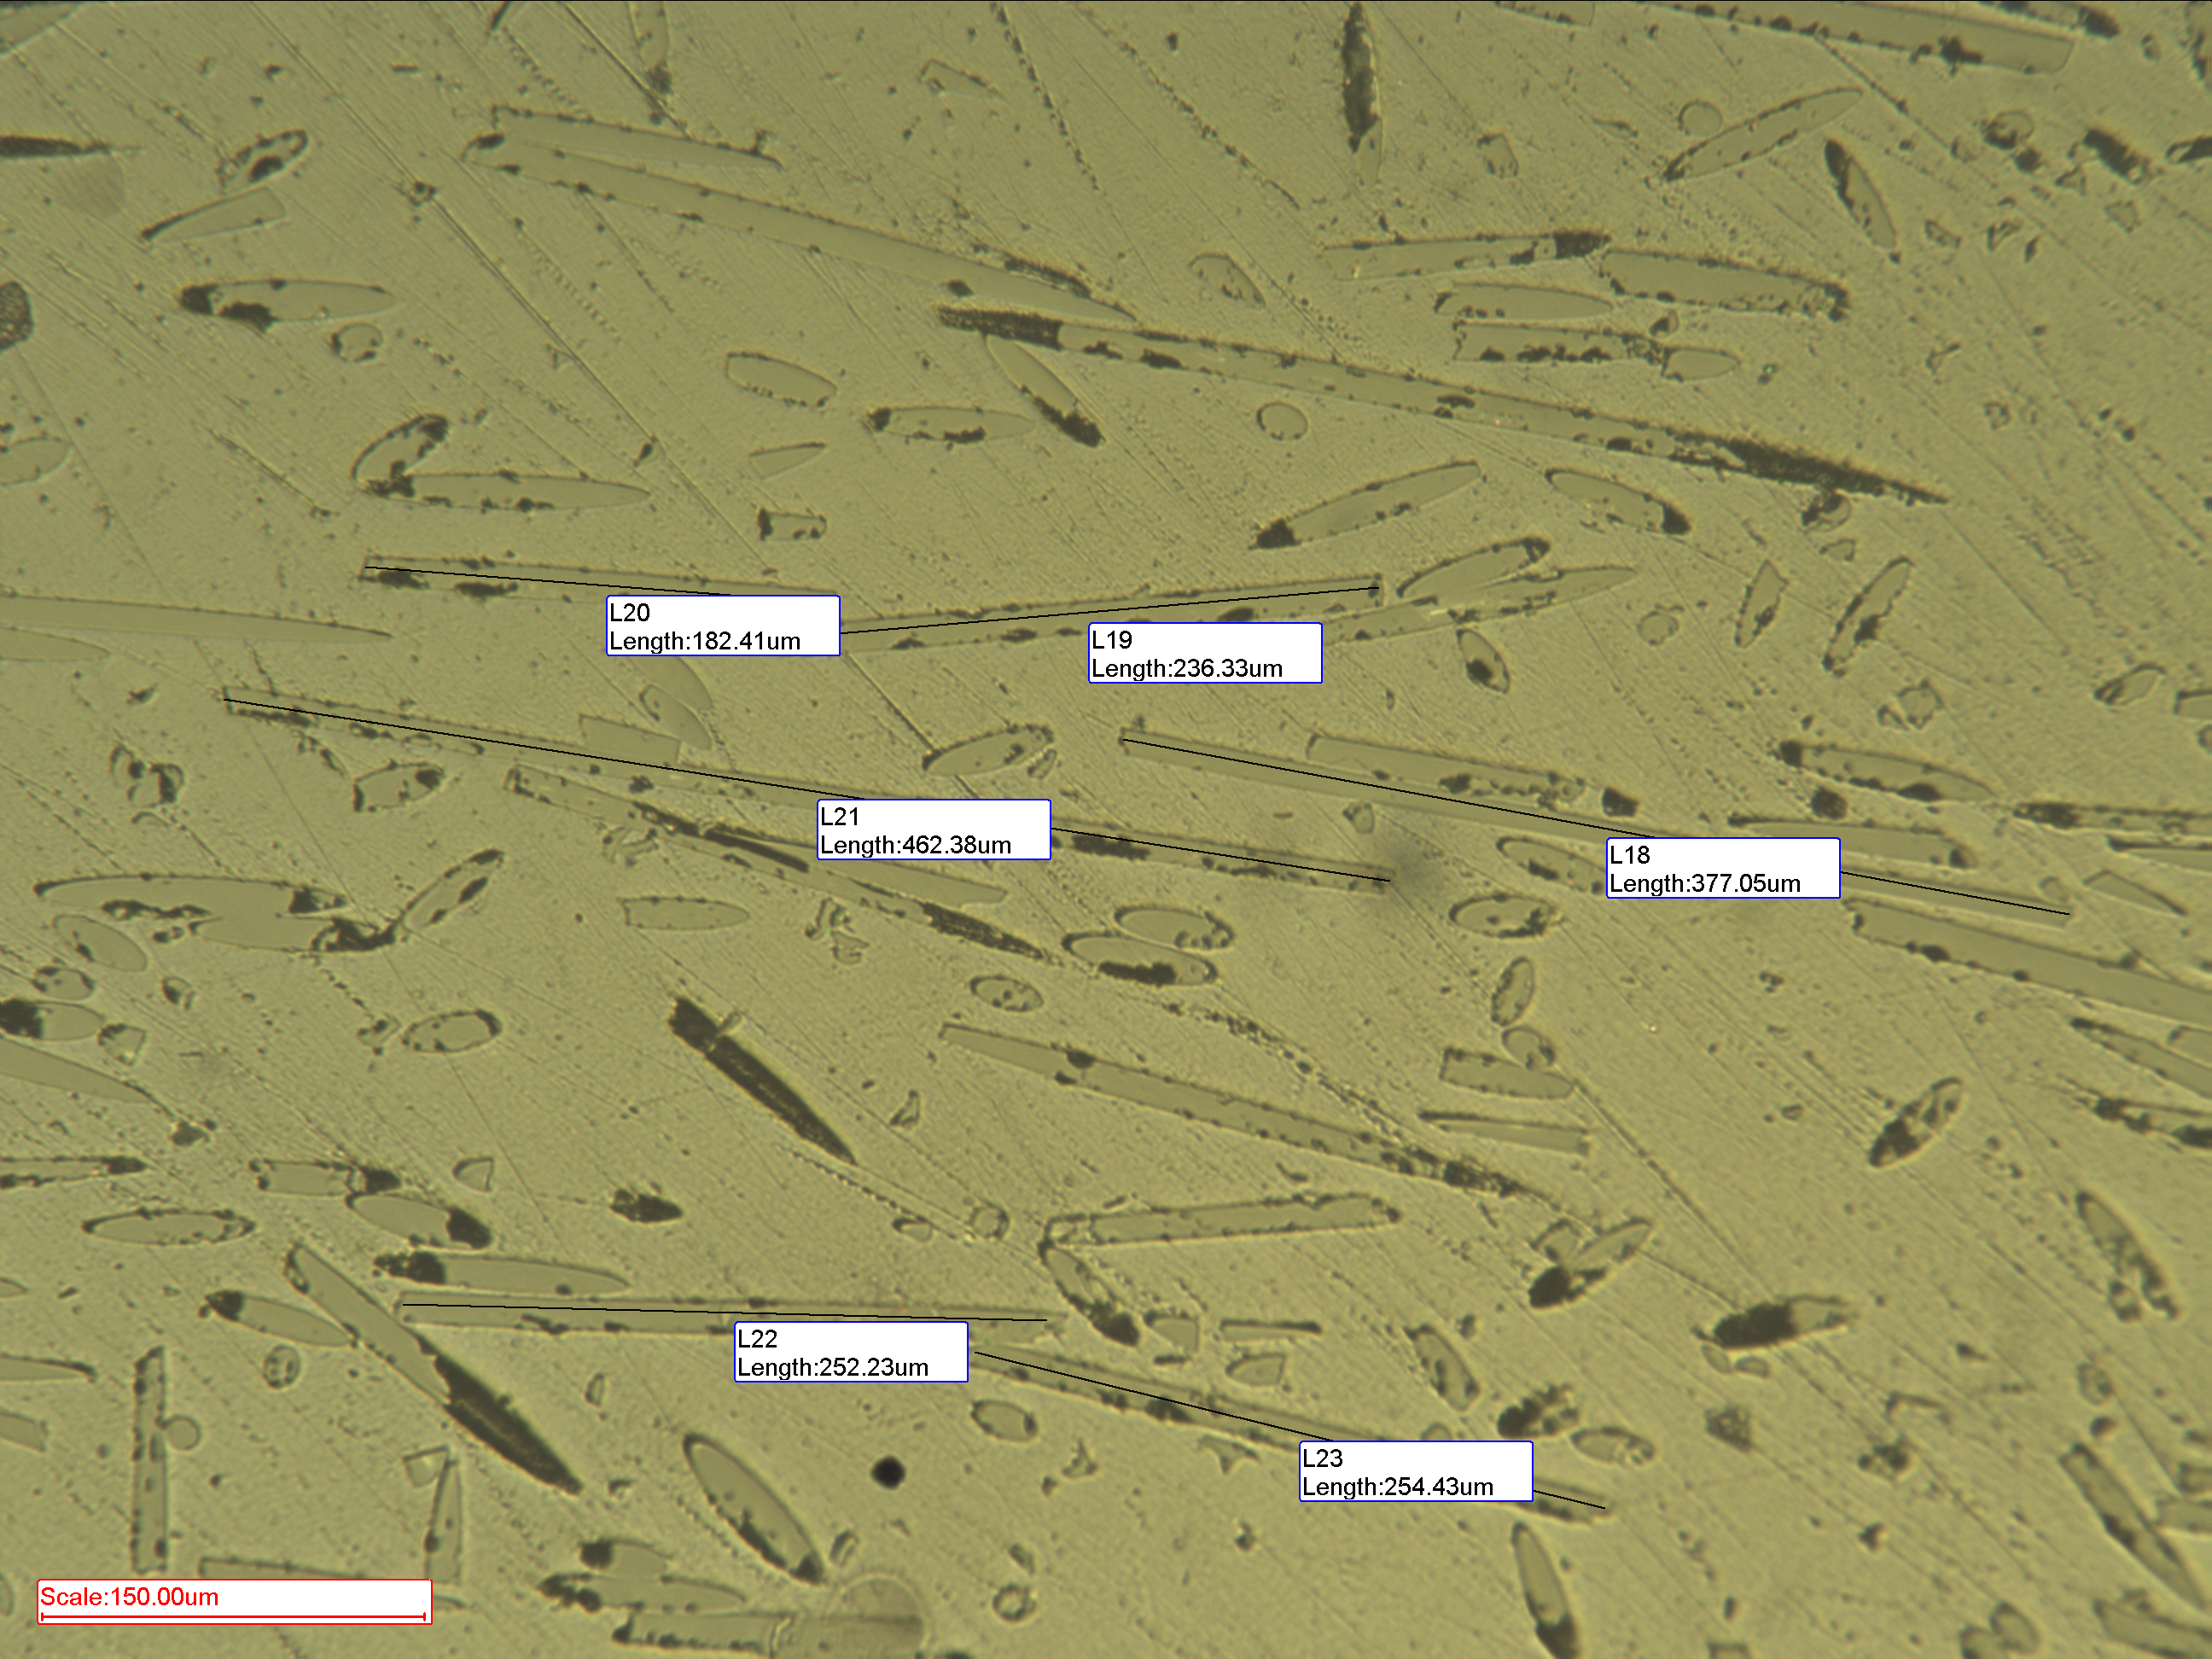
\includegraphics[width=.7\linewidth]{figures/PBT11_Long.png}
\caption{PBT11 Longitudinal Fiber Counting}
\label{pbt11longcount}
\end{figure}
\begin{figure}[H]
\centering
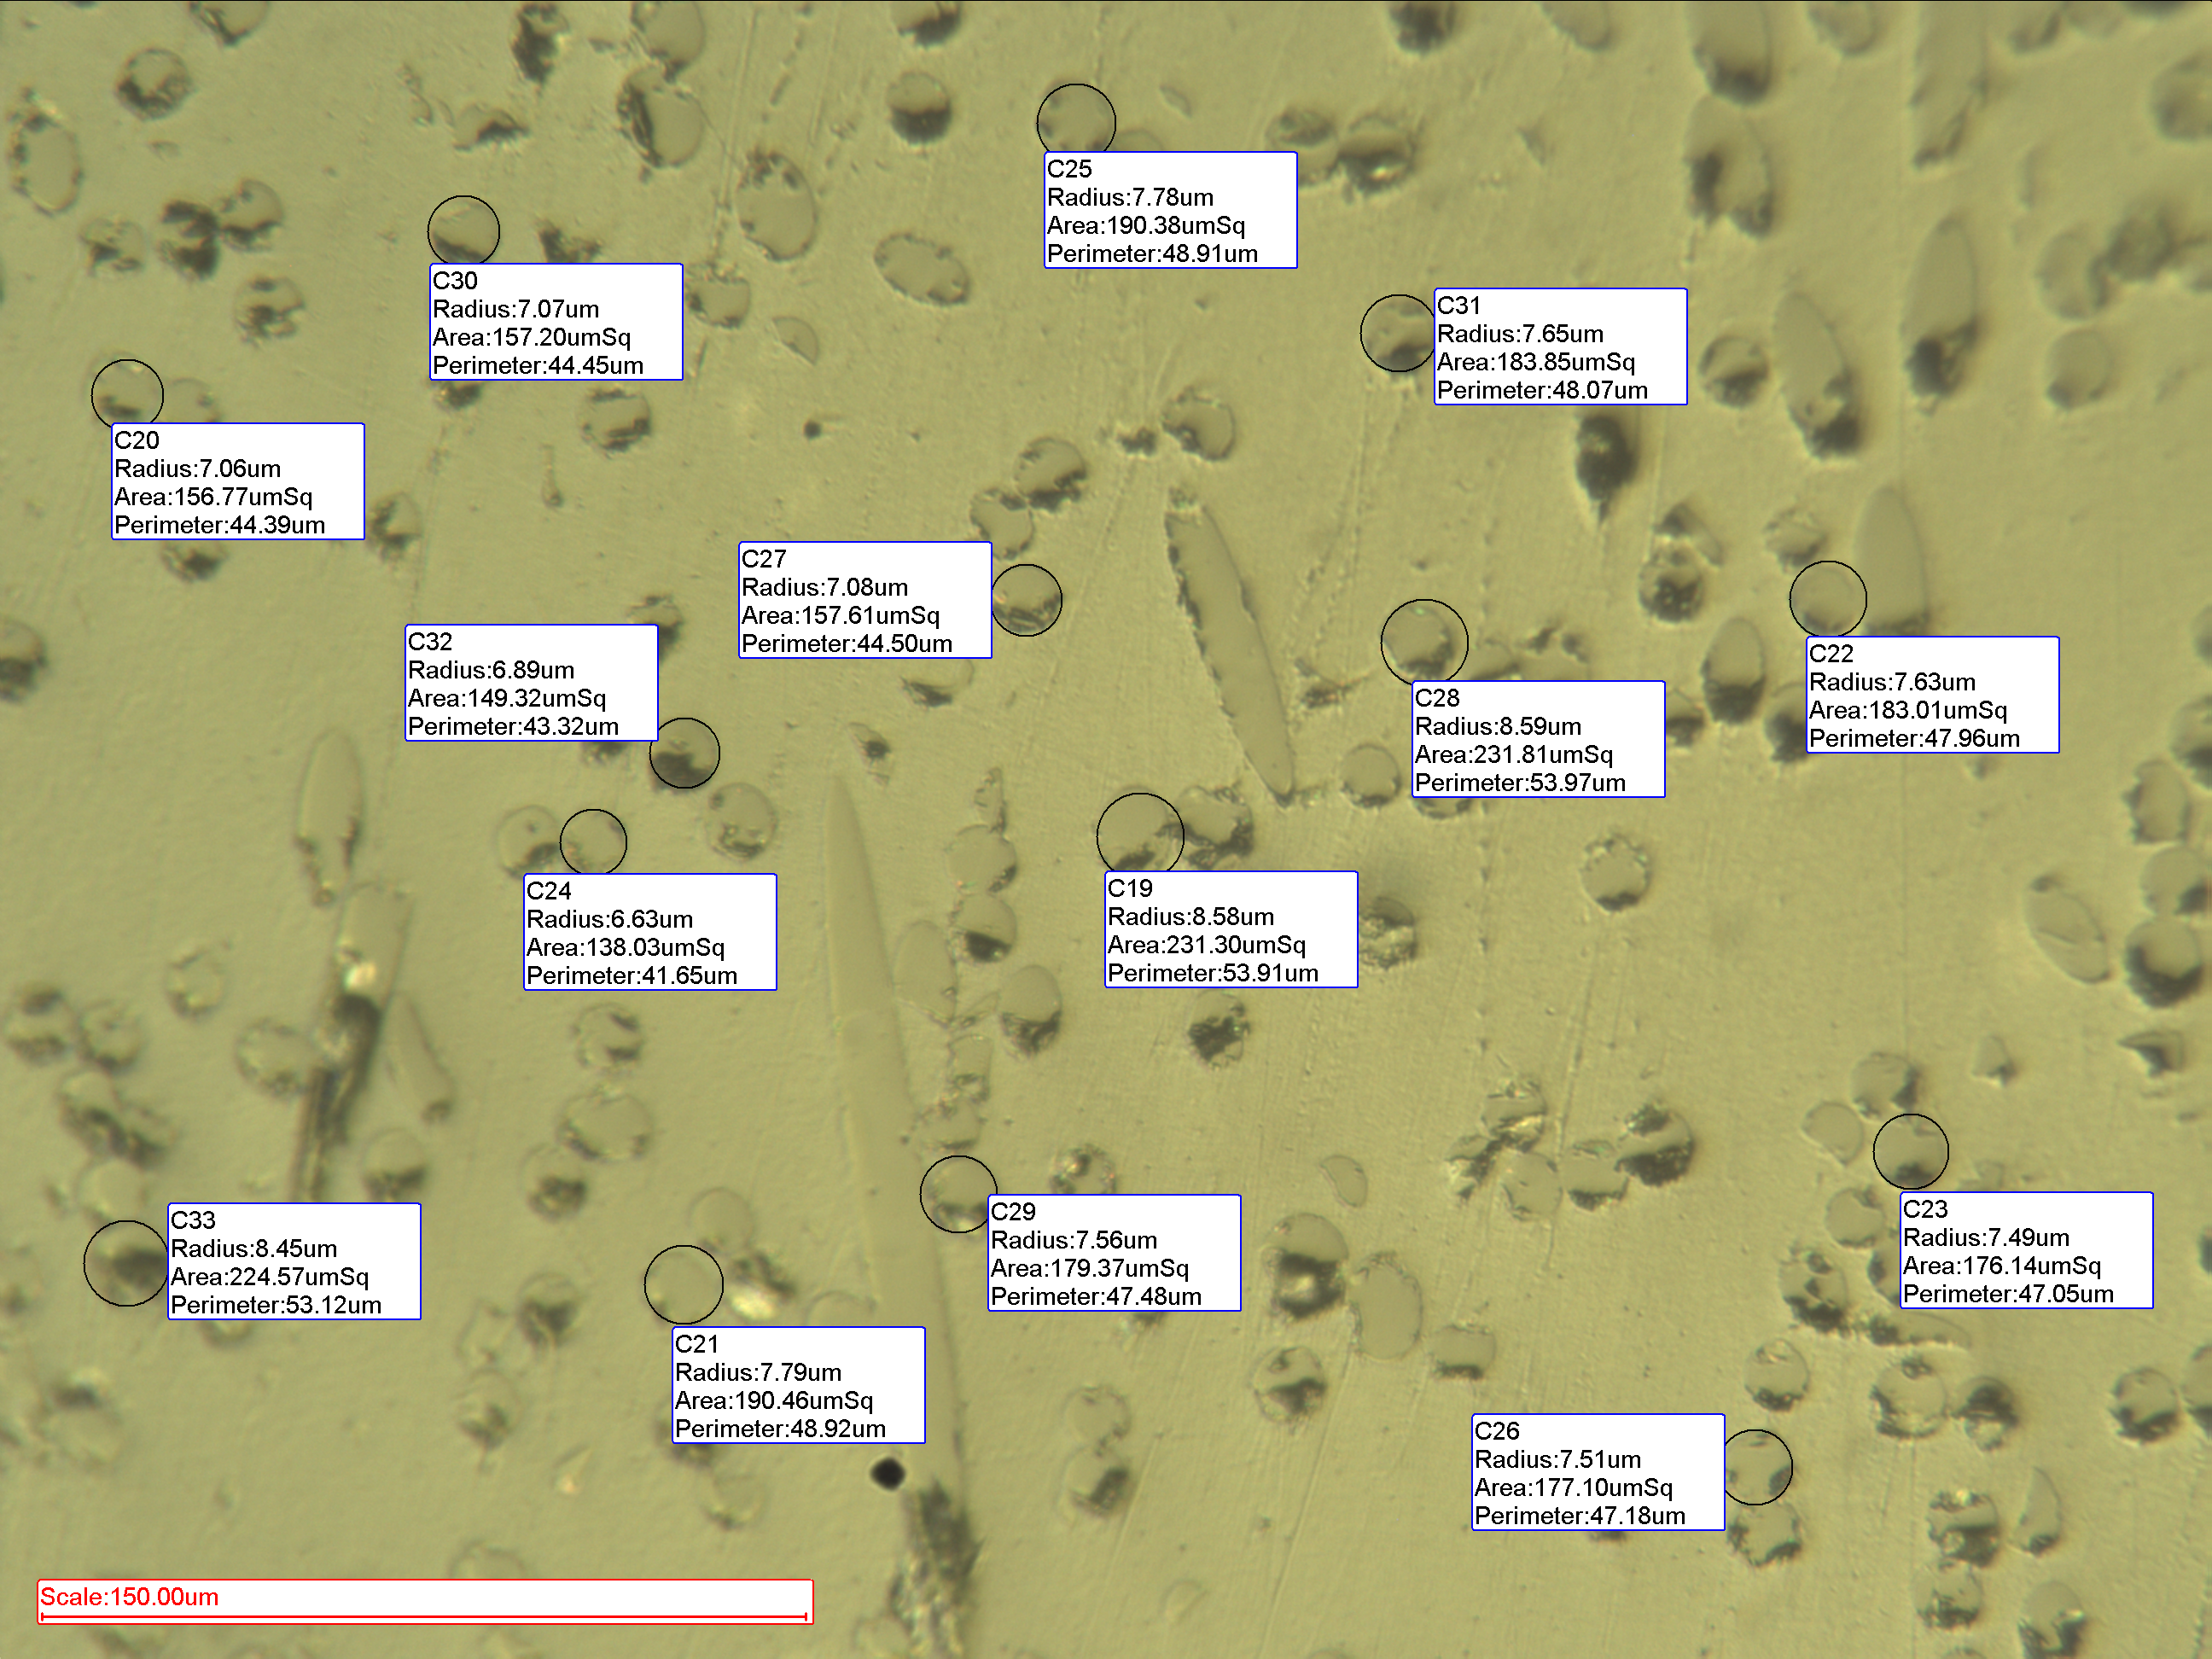
\includegraphics[width=.7\linewidth]{figures/PBT11_Trans.png}
\caption{PBT11 Transverse Fiber Counting}
\label{pbt11transcount}
\end{figure}
\begin{figure}[H]
\centering
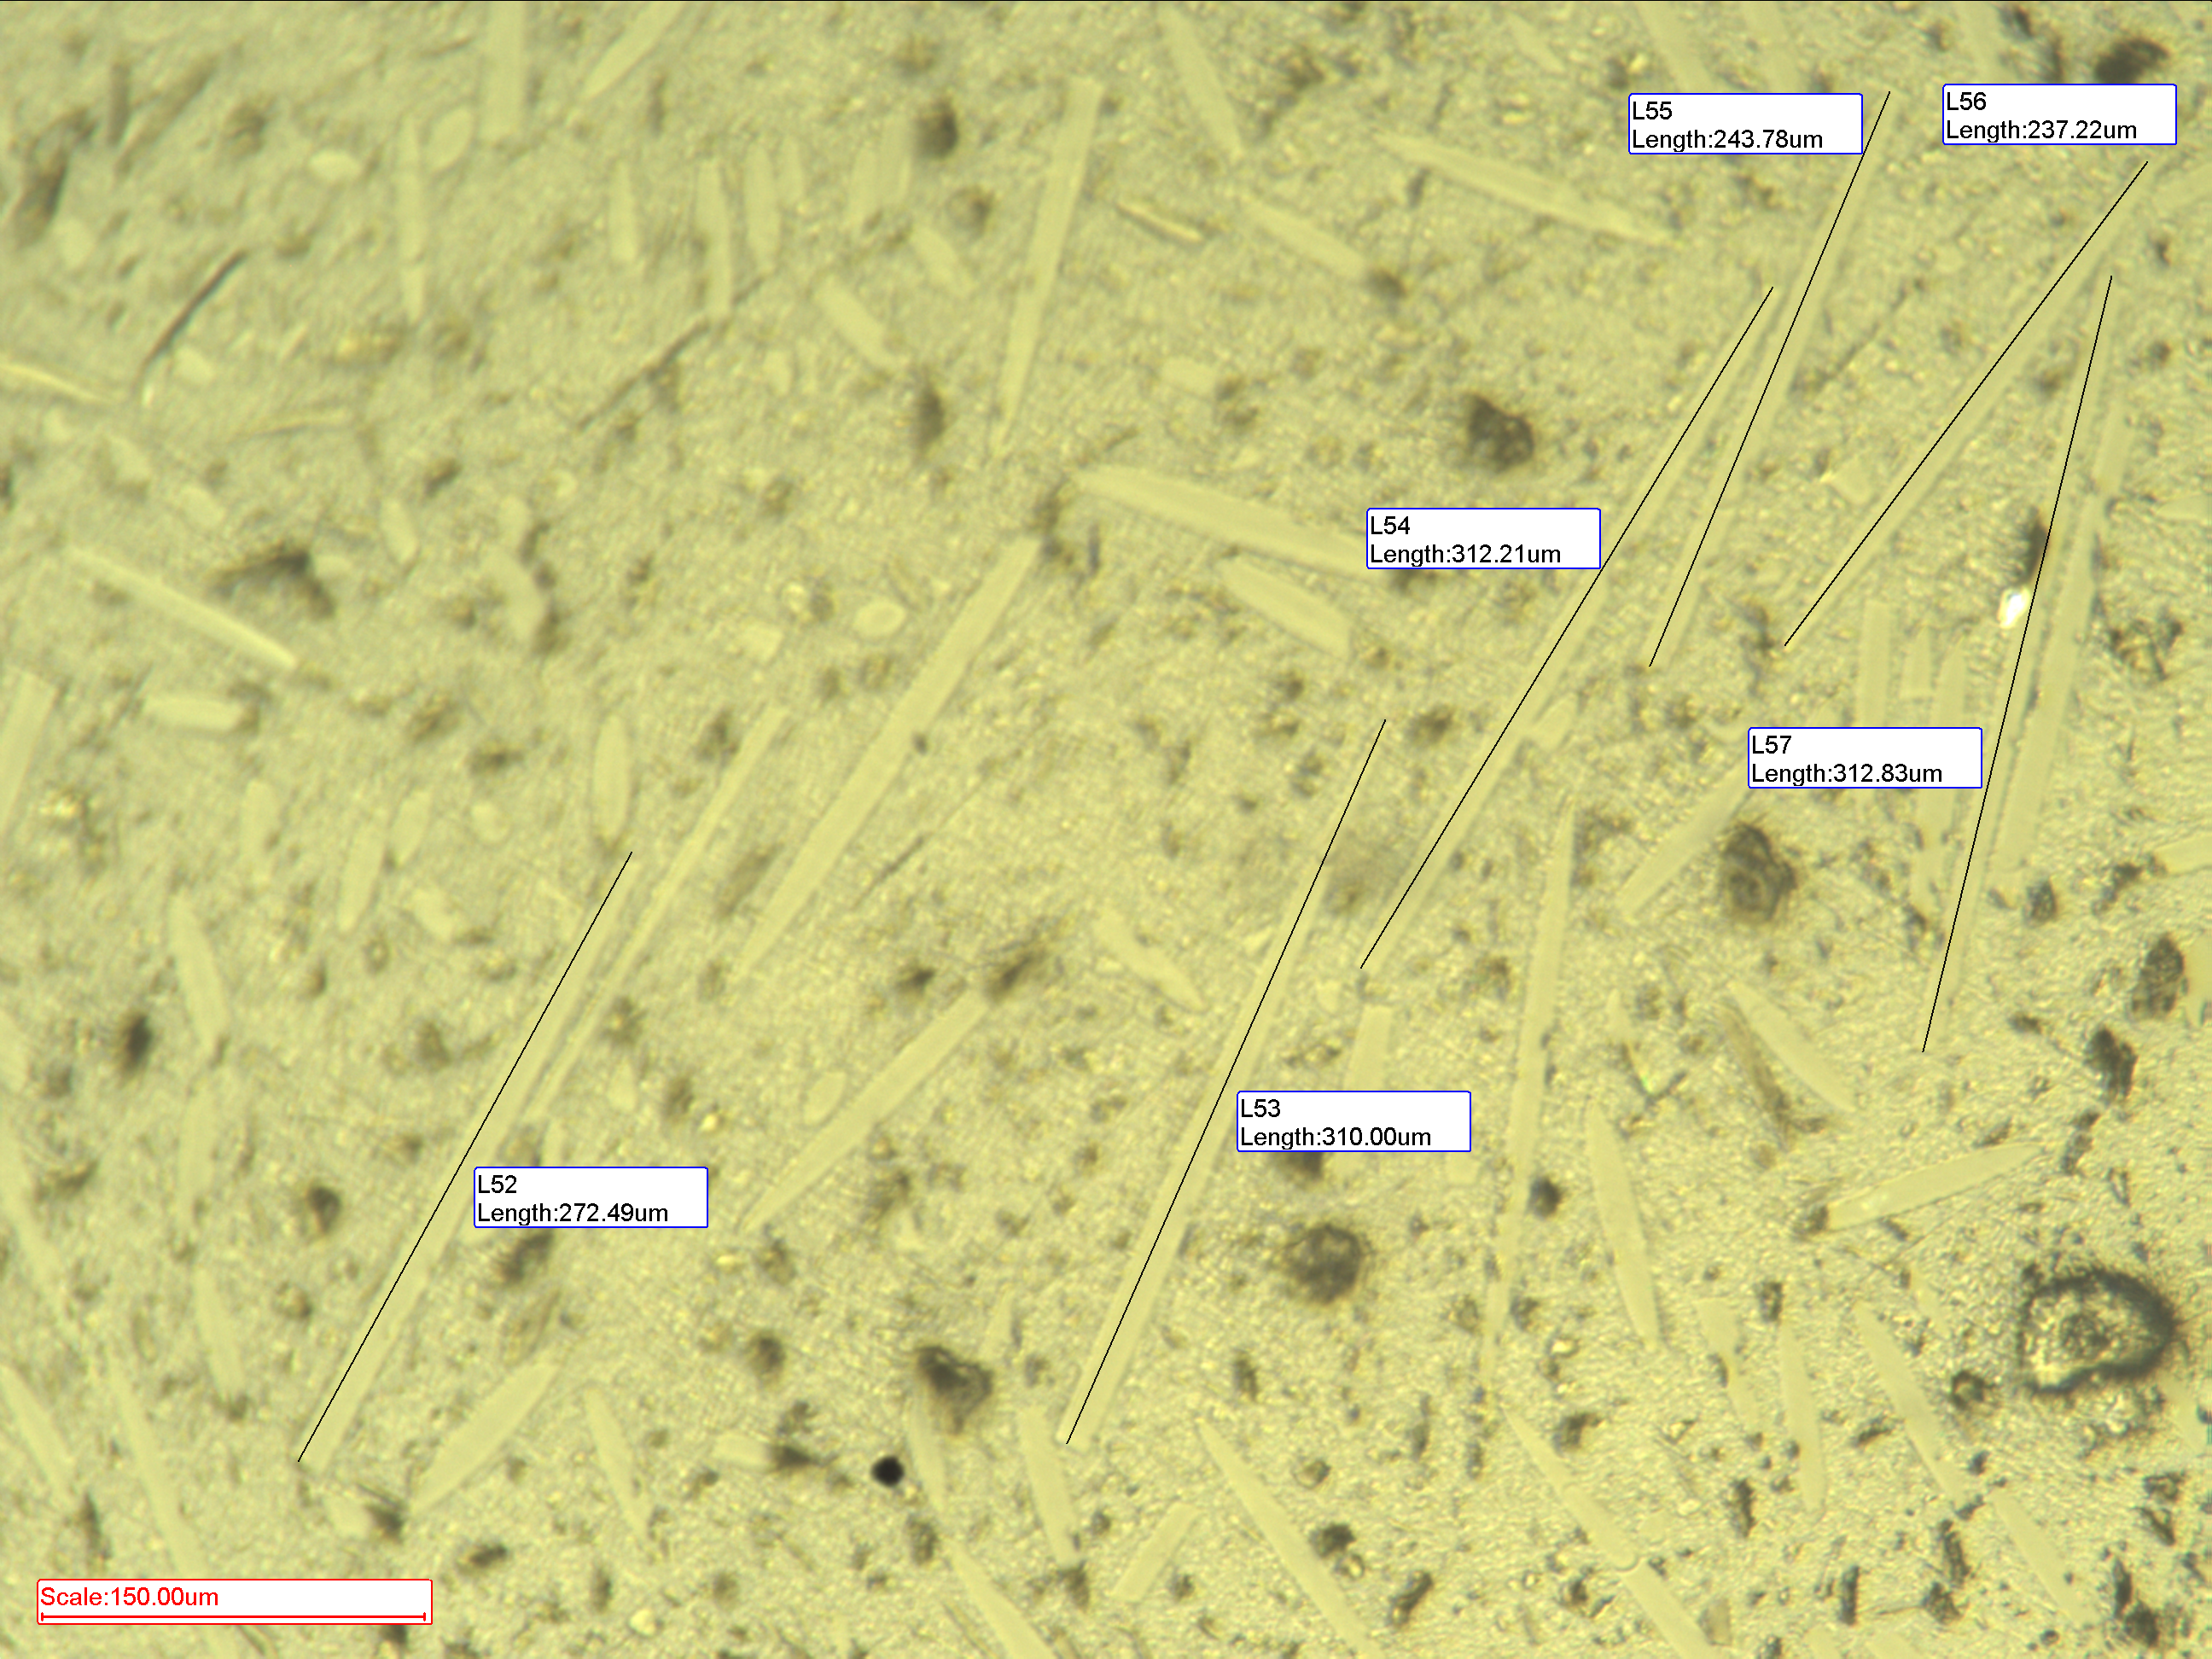
\includegraphics[width=.7\linewidth]{figures/PBT12_Long.png}
\caption{PBT12 Longitudinal Fiber Counting}
\label{pbt12longcount}
\end{figure}
\begin{figure}[H]
\centering
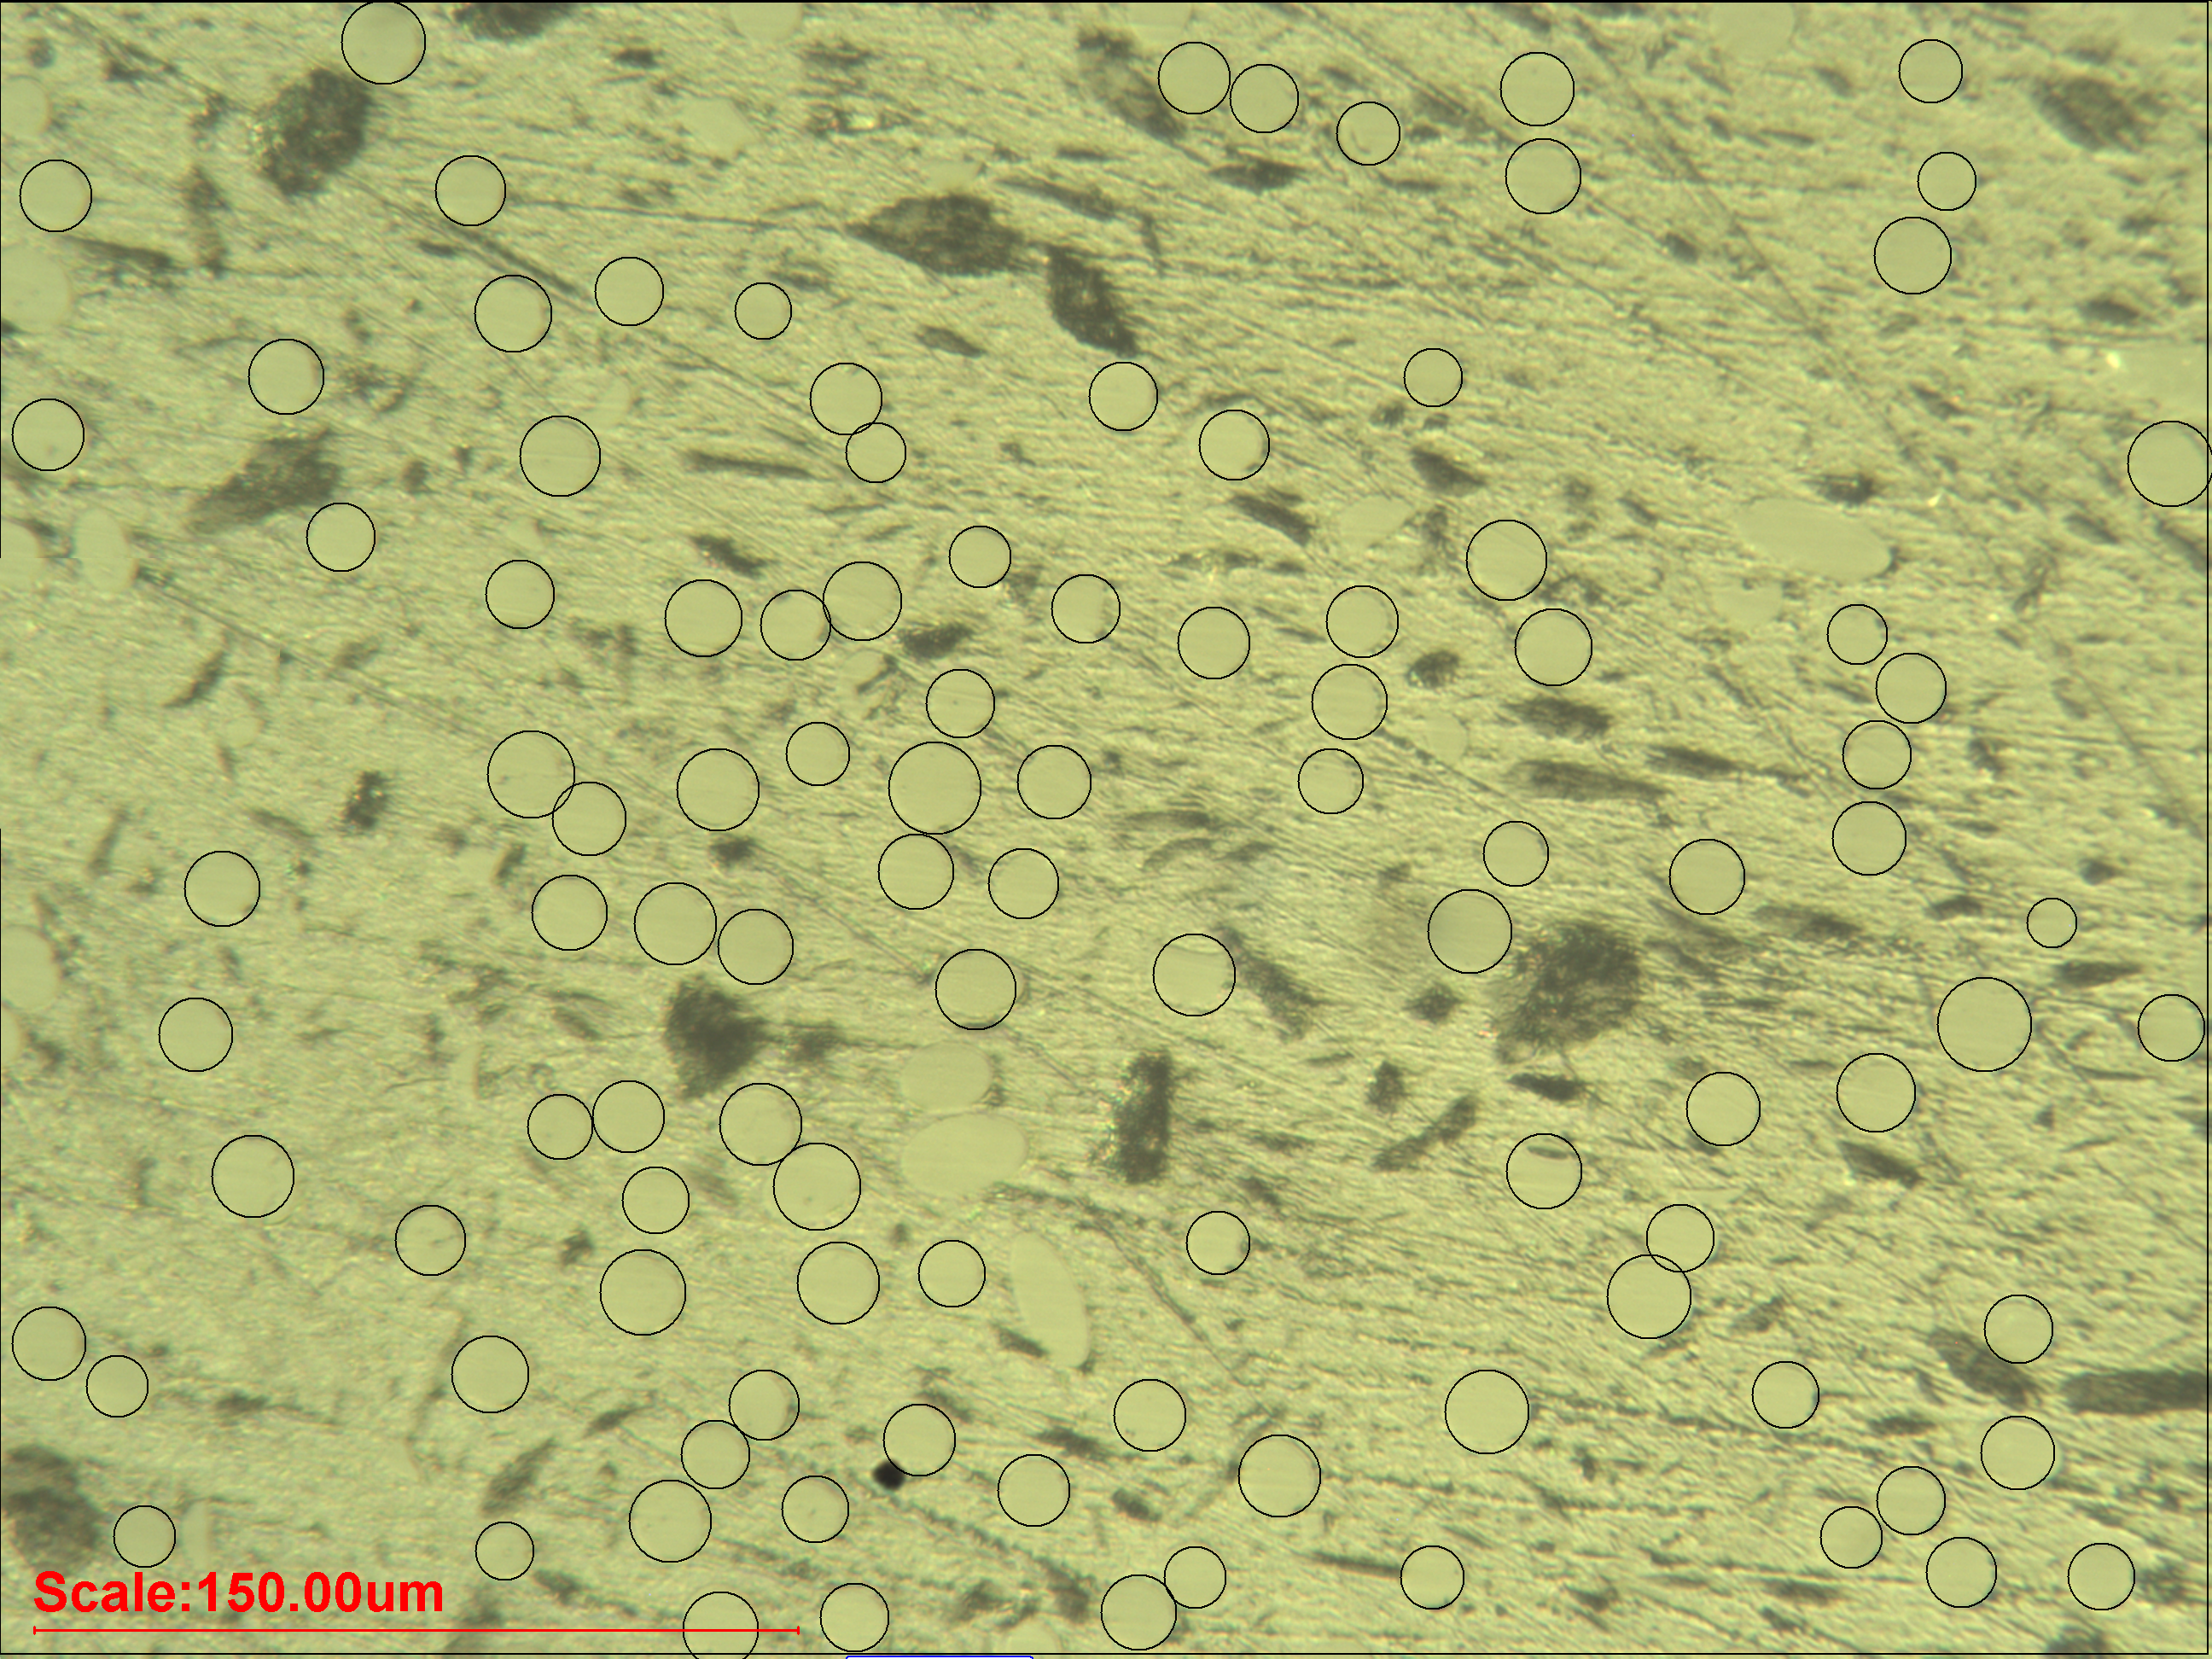
\includegraphics[width=.7\linewidth]{figures/PBT-12-TRANSVERSE-COMBINED.png}
\caption{PBT12 Transverse Fiber Counting}
\label{pbt12transcount}
\end{figure}

\begin{figure}[H]
\centering
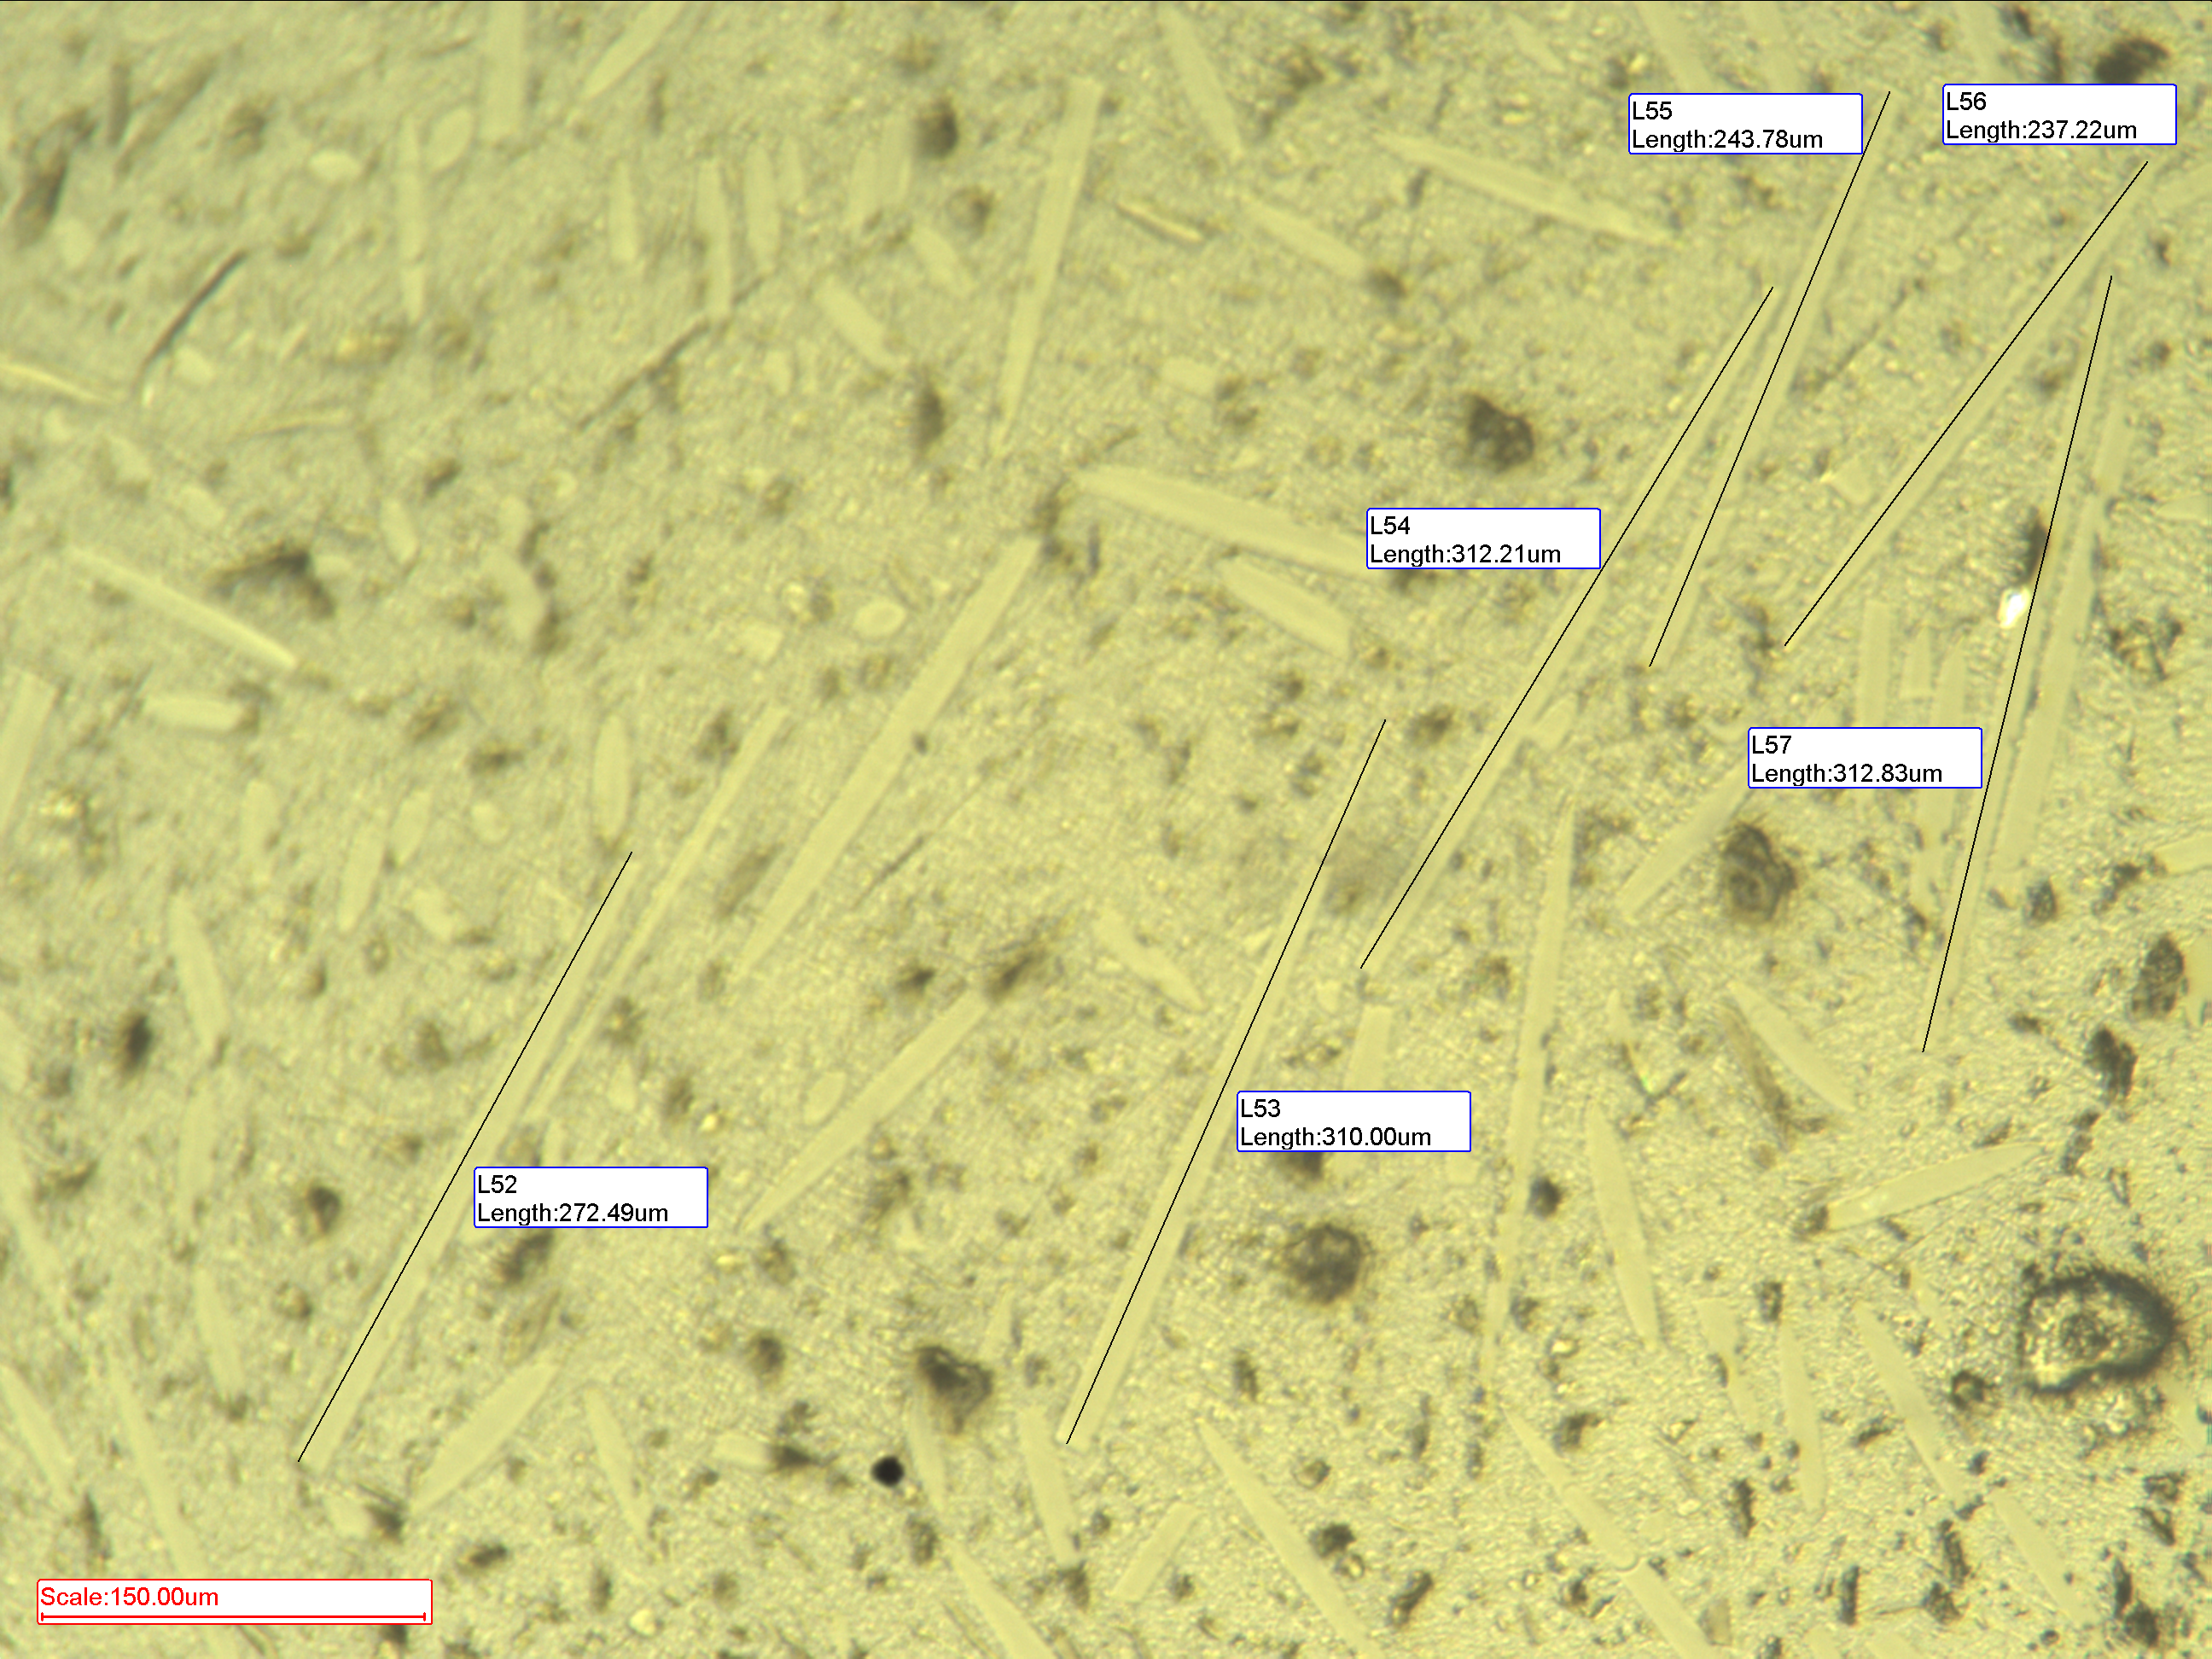
\includegraphics[width=.7\linewidth]{figures/PBT12_Long.png}
\caption{PBT14 Material}
\label{pbt12longcount}
\end{figure}

Table \ref{tab:MeasuredValues} lists the respective values for PBT9, PBT11, PBT12, and PBT14. For PBT9 it was assumed that the fibers used in the composite would be the same as PBT11 and PBT12. The fiber lengths and diameters were simply calculated as the respective average of the same values for PBT11 and PBT12.  Note that the values for PBT9 fiber length and diameter are averaged from the values found for PBT11 and PBT12.

It can also be noted that in the microscope pictures for PBT12, there are visible ``dark spots`` which could possibly be voids, irregularities in the matrix or foreign material which may have contaminated the sample. This is noted in the lab orientation. Comparably, looking at PBT11, there is a smaller amount of voids and if there are voids seen, they are much smaller than that in PBT12. The presence of voids or contaminants can have undesirable effects on the overall strength of the composite and are discussed later in this report. 

Since PBT14 had no fibers in the polymer, these values were ignored, or set to zero.
\onehalfspacing
\begin{center}
\captionof{table}{Microscope Analysis PBT9, PBT11, PBT12, and PBT14 Values} \label{tab:MeasuredValues}
\begin{tabular}{p{1.5cm} || p{3.cm} | p{3.cm} | p{3.cm} | p{2.cm}}
\hline
Sample & \multicolumn{1}{c|}{PBT9} & \multicolumn{1}{c|}{PBT11} & \multicolumn{1}{c|}{PBT12} & \multicolumn{1}{c}{PBT14} \\
\hline
\hline
\(V_f\) & 0.224 & 0.179 & 0.135 & 0\\
\(V_m\) & 0.78 & 0.82 & 0.86 & 1 \\
\(\ell (\mu m)\) & 294.14 & 299.33 & 288.94 & N/A\\
\(d (\mu m) \) & 14.61 & 14.60 & 14.61 & N/A\\
\(\ell /d\) & 20.14 & 20.50 & 19.77 & N/A\\
\(V_v\) & N/A & Few,small voids & Many,larger voids or irregularities & No voids\\
\hline
\end{tabular}
\end{center}

\subsection{Tensile Tests}
The figures found in Appendix A graph the tensile tests performed for samples of PBT9, PBT11, PBT12, and PBT14 in the elastic regions and up to fracture using the provided instron data. As expected, PBT9, 11 and 12 exemplify a composite behaviour, following a linear trend upwards in stress until a fracture point. It is also obvious from the stress-strain curve of PBT14  that the response is of a polymer until failure. The material yields and the stress drops down to a necking region until fracture after a certain amount of strain.

Observing these graphs, it is clear that the modulus is fairly consistent for each of the PBT samples, but when it comes to the fracture point, the test samples performed slightly differently. For PBT9, the fracture strength ranged from 97MPa up to 112MPa, with a strain at break of 4\% to 6\%. For PBT11, the data is more precise, with the fracture strength ranging from 110MPa to 113MPa, with a strain at break of 5\% to 6\%. For PBT12, the data is also fairly precise, with the fracture strength ranging from 60MPa to 67MPa, with a strain at break of 4.5\% to 5\%. Finally, PBT14 had precise fracture strengths (31MPa to 34MPa), but very diverse strains at break (40\% to 130\%). These values are used later on for comparison against analytical results and so the averages of the three samples for each test are tabulated in Table \ref{tab:TestValues}. The experimental values for PBT14 are also used for further calculations which require matrix yield strength and fracture strength.

\begin{center}
\captionof{table}{Summary of Average Tensile Test Data} \label{tab:TestValues}
\begin{tabular}{p{1.5cm} || p{5.cm} | p{5.cm} | p{1.5cm} }
\hline
Sample & \multicolumn{1}{c|}{Young's Modulus (MPa)} & \multicolumn{1}{c|}{Fracture Stress (MPa)} & \multicolumn{1}{c}{\(V_f\)}  \\
\hline
\hline
PBT9 & 13448 & 107.01 & 0.224\\
PBT11 & 10180.33  & 111.94 & 0.179\\
PBT12 & 11957 & 65.31 & 0.135 \\
PBT14 & 2558 & 33.65 & 0\\
\hline
\end{tabular}
\end{center}
\singlespacing

\subsection{Fiber and Matrix Data}
Table \ref{tab:MaterialValues} shows the mechanical material properties of the fiber (E-Glass) and matrix (PBT) materials which are averages taken from the material properties presented in the introduction \cite{PBTmechProperties} \cite{course_notes}. These will be used later on when calculating the Young's Modulus and Fracture Stress of the samples. The Young's Modulus for PBT is determined from Figure \ref{pbt14tensile} and the fracture strength and yield stress for PBT is obtained from observing the yield points of Figure \ref{pbt14fail} in Appendix A.

\newpage
\begin{center}
\captionof{table}{Material Data for E-Glass Fiber and PBT Polymer} \label{tab:MaterialValues}
\begin{tabular}{p{2.5cm} || p{3.cm} | p{4.cm} | p{2.5cm} | p{1.cm} }
\hline
Material & Young's Modulus (MPa) & \(\sigma^*\), Fracture Strength (MPa) & Shear Modulus (MPa) & Yield (MPa)\\
\hline
\hline
\(E-Glass\) \cite{course_notes} & 70000 &  3400 & 881.6 & N/A \\
\(PBT\) \cite{PBTmechProperties} & 2558 & 33.65 & N/A & 60.91\\
\hline
\end{tabular}
\end{center}
\singlespacing

\section{Discussion}

\subsection{Assumptions}
Using the values in Table \ref{tab:MeasuredValues} and Table \ref{tab:MaterialValues} the elastic modulus of the samples can be found using both the Halpin approach (Equation \ref{eq:halpin}) and simple equation (Equation \ref{eq:simple}). First, it is helpful to determine which set of equations are valid for this case. We assume for these calculations that the fibers are short, discontinuous and parallel to the load direction as seen through the pictures on the microscope. From this we can select the equations which are presented below. 

It is also assumed for using the following fracture stress and Young's Modulus equations that:

\begin{itemize}
\item All fibers are the same length
\item All fibers are perfectly parallel to the load direction (unidirectional)
\item The processing of the fibers during the production of the composite is done so that the bond between fiber and matrix is perfect. (Imperfections such as the presence of excess moisture that could lead to poor adhesion)
\item There are no voids present in the matrix
\end{itemize}

Further assumptions are made for doing calculations for the Young's Modulus which relate to the stress conditions in the matrix and fiber.

\begin{itemize}
\item Iso-stress condition. The stress in the fiber is the same as the stress in the matrix.
\item Poisson contractions for the matrix and fiber are ignored
\end{itemize}

These assumptions are used to explain the sources of error later in the report when comparing the experimental results against analytical, rule of mixtures equations.

% need reference for this

\subsection{Young's Modulus - Halpin Approach}

To calculate \(E_{\downarrow \downarrow}^{short}\) using the Halpin method, two variables are required, \(\eta\) and \(\xi\). These variables try to estimate the composite geometry and arrangement of fibers in the matrix. These are calculated using equations [2.3(24)] and [2.3(25)] respectively from the course notes \cite{course_notes}.

\begin{equation}
\eta = \frac{E_f/E_m-1}{E_f/E_m+\xi}
\end{equation}

\begin{equation}
\xi = 2 \frac{l}{d} +40V^{10}_f
\end{equation}

The values for the Young's Modulus of the fiber and the matrix can be found in Table \ref{tab:MaterialValues} and the ratio of  length, \(\ell\), over diameter, \textit{d} is the aspect ratio which is an important paramater determined from the results of measuring the fibers and diameters from Table \ref{tab:MeasuredValues}. Once these parameters are found, equation [2.3(26)] from the course notes is used to determine the Young's Modulus for short, discontinuous fibers \cite{course_notes}.

\begin{equation} \label{eq:halpin}
\frac{E^{short}_{\downarrow \downarrow}}{E_m} = \frac{1+\xi \eta V_f}{1-\eta V_f}
\end{equation}

\subsection{Young's Modulus - Simple Approach}

The simple method of calculating \(E_{\downarrow \downarrow}^{short}\) is a method developed by H.L. Cox whose equation can be found in the course notes as [2.3(23)] \cite{course_notes}.

\begin{equation} \label{eq:simple}
E^{short}_{\downarrow \downarrow} = \eta_l E_f V_f + E_m(1-V_f)
\end{equation}

The simple method is developed from the rule of mixtures for a unidirectional lamina and applying a length correction factor, \(\eta_l\) which is found using equations [2.3(24)] and [2.3(25)] from the course notes \cite{course_notes}. The simple approach tries to estimate the composite geometry as well, but uses interfiber spacing instead of an aspect ratio as used in the Halpin equations.

\begin{equation}
\eta_l = 1- \left[\frac{\tanh 0.5\beta l}{0.5\beta l} \right]
\end{equation}

\begin{equation}
\beta=\left[\frac{2G_m}{E_fr^2 ln(\frac{R}{r})}\right]^{1/2}
\end{equation}

The shear modulus for the matrix can be found in Table \ref{tab:MaterialValues}. The ratio of interfiber spacing, \textit{R} and fiber radius, \textit{r} can be found using the following equation from Hull \cite{hull}. This relationship is for hexagonally arranged fibers but because the ratio of \(\frac{R}{r}\) appearing in a logarithmic term in \(\beta\) , the hexagonal arrangement is acceptable to use as the result of the logarithmic term is sufficiently insensitive to fiber arrangement.

\begin{equation}
\frac{1}{V_f}=\left[\frac{R}{r}\right]^2
\end{equation}

\subsection{Fracture Strength Calculation}

The fracture strength equations rely on the \textit{critical fiber length}, \(\ell_c\), which is minimum length of fiber that is required to build up tensile stresses up in the fiber to the fracture strength. This is calculated using equation [2.4(32)] from the course notes \cite{course_notes}.

\begin{equation}
\ell_c = \frac{\sigma^*_f r}{\tau^*_i}
\end{equation}

The interfacial shear strength, \(\tau^*_i\), is found to be equal to the shear yield of the matrix, \(\tau^y_m\), which is determined by

\begin{equation}
\tau^*_i = \tau^y_m = 0.5 \sigma^y_m
\end{equation}

The value for the yield strength for the matrix can be found from the stress-strain curve of the matrix until failure Figure \ref{pbt14fail} in the Appendix to be 60.91 MPa. This is used since it known that after the polymer yields, it will go into plastic deformation and neck until failure. This value falls near the range of the yield stress documented for PBT from online sources.

\begin{center}

\(\tau^*_i = \tau^y_m = 0.5(60.91)\)
\\
\(\tau^*_i = \tau^y_m = 30.46 MPa\)

\end{center}

The \textit{critical fiber length} for the PBT samples are approximately 815 microns, and since the average fiber lengths found in the samples (Table \ref{tab:MeasuredValues}) are less than the critical length, it is valid to use equation [2.4(44)] from the course notes \cite{course_notes} for fractures stress of the composite. 

\begin{equation} \label{eq:fracture}
\sigma^*_{\downarrow \downarrow} = \left( \frac{l}{2l_c}\right) \sigma_f^* V_f + \sigma^*_m V_m
\end{equation}

The values for the fiber and matrix fracture strength can be found in Table \ref{tab:MaterialValues}.

\subsection{Analytical Values}

The results of the prior calculations are shown in the following table. The calculations show that there is a small difference of up to 6\% between calculations done using the Halpin approach versus those done using the simple calculation approach. Note that there is no difference between methods for PBT14 since it has no fibers and result in just the matrix young's modulus for both equations.

It will be shown in the next section that the Young's Modulus values are much closer to the experimental results than the fracture strength values are.

\begin{center}
\captionof{table}{PBT9, PBT11, PBT12, and PBT14 Modulus and Fracture Stress} \label{tab:CalculatedValues}
\begin{tabular}{p{3.5cm} || p{2.cm} | p{2.cm} | p{2.cm} | p{2.cm}}
\hline
Sample & \multicolumn{1}{c|}{PBT9} & \multicolumn{1}{c|}{PBT11} & \multicolumn{1}{c|}{PBT12} & \multicolumn{1}{c}{PBT14} \\
\hline
\hline
\(E^{short}_{\downarrow \downarrow}\) Halpin (MPa)& 12658.3 &  10508.06 & 8376.91 & 2558\\
\(E^{short}_{\downarrow \downarrow}\) Simple (MPa)& 12256.6 & 10366.57 & 8338.3 & 2558\\
\hline
Halpin vs. Simple, \% Difference & 6.07 & 5.12 & 3.18 & 0\\
\hline
\(\sigma^*_{\downarrow \downarrow}\) (MPa)& 163.50 & 139.19 & 110.30 & 33.65\\
\(\ell_c (\mu m) \) & 815.28 & 814.93 & 815.64 & N/A\\
\hline

\end{tabular}
\end{center}
\singlespacing

\subsection{Rule of Mixtures Applicability}

\subsubsection{Young's Modulus}

The results of the calculations using the Halpin and simple approach are taken and plotted and compared against the experimental values of the Young's Modulus. The following graph and Table \ref{tab:ComparingModulus} shows how closely the calculated values are to the experimental. Note that PBT14 has no error since its modulus was used in the calculation for the rest of the materials.

\begin{figure}[H]
\centering
\includegraphics[width=.95\linewidth]{figures/modulus_test_vs_calc.png}
\caption{Young's Modulus, Experimental vs. Analytical}
\label{ModulusCompare}
\end{figure}

\begin{center}
\captionof{table}{Comparison of Young's Modulus for Experimental vs. Analytical Calculations} \label{tab:ComparingModulus}
\begin{tabular}{p{1.25cm} || p{1.5cm} | p{1.5cm} | p{1.5cm} | p{1.5cm} | p{1.5cm} | p{1.5cm}}
\hline
 \multirow{2}{*}{Sample} & \multicolumn{5}{c|}{Young's Modulus (MPa)} & \multirow{2}{*}{\(V_f\)} \\
   &  \multicolumn{1}{c}{Test} & \multicolumn{1}{c}{Halpin} & \multicolumn{1}{c}{\% Error} & \multicolumn{1}{c}{Simple} & \multicolumn{1}{c|}{ Error} \\
\hline
PBT9 & 13448 & 12658.33 & 6.24 & 13426.83 & 0.16 & 0.224\\
PBT11 & 10180.33 & 10508.06 & 3.12 & 11046.50 & 7.84 &  0.179\\
PBT12 & 11957 & 8376.91 & 42.74 & 8651.73 & 38.20 & 0.135 \\
PBT14 & 2558 & 2558 & 0 & 2558 & 0 & 0\\
\hline
\end{tabular}
\end{center}
\singlespacing

As mentioned before, the tensile test data for PBT12 was collected incorrectly and lead to erroneous results for the experimental Young's Modulus value. Therefore, for the Halpin equations, PBT12 has the largest error of 42.74\%. The rest of the analytical values for PBT9 and PBT11 are within a 6\% error of the experimental values. It can be seen from Figure \ref{FScompare} that as you go from PBT14 which contains no fibers to PBT12, 11 and  9, the Young's Modulus increases. This is attributed to the increasing volume fraction of E-Glass fibers. This can be clearly seen from the relationship in Equation \ref{eq:simple} for the calculation of Young's Modulus using the simple approach. The experimental values should also show the same trend as the analytical values, but again, because of the error with testing PBT12, it shows a higher Young's Modulus than that of PBT11 which is not to be expected. 

When calculating the Young's Modulus, there is some discrepancy between the Halpin approach and the simple approach. Both approaches try to use the distribution and geometry of fibers to determine the overall Young's Modulus of the resulting composite. The simple method utilises a correction factor, \(\eta_l\), based on the fiber packing geometry to estimate the microstructure of the composite while the Halpin approach uses the aspect ratio, \(\frac{\ell}{d}\). The calculated values and error for both as displayed in Table \ref{tab:ComparingModulus} show that the simple method was better at estimating the modulus for PBT9 and PBT12 (if it were a correct value) but worse than Halpin at estimating PBT11 modulus. Doing an R\textsuperscript{2} regression analysis of each of the methods with the experimental results show that using the simple method performed better in terms of estimating the Young's Modulus.

\begin{equation}
R^2_{Halpin} = 0.9683
\end{equation}

\begin{equation}
R^2_{Simple} = 0.9727
\end{equation}

Error with these calculations, especially in PBT12, compared to the experimental data can be attributed to the assumptions that all the fibers are the same length, are unidirectional and are bonded perfectly to the matrix. This is discussed in the verification section.

\subsubsection{Fracture Strength}

The fracture strength results of the experimental are plotted against the analytical calculation below. Note that PBT14 has no error since its modulus was used in the calculation for the rest of the materials.

\begin{figure}[H]
\centering
\includegraphics[width=.95\linewidth]{figures/fracture_stress_test_vs_calc.png}
\caption{Fracture Strength, Experimental vs. Analytical}
\label{FScompare}
\end{figure}


\begin{center}
\captionof{table}{Comparison of Fractures Stress for Experimental vs. Analytical Calculations} \label{tab:ComparingFracture}
\begin{tabular}{p{1.25cm} ||  p{1.5cm} | p{1.5cm} | p{1.5cm} | p{1cm}}
\hline
 \multirow{2}{*}{Sample} & \multicolumn{3}{c|}{Fracture Stress (MPa)} & \multirow{2}{*}{\(V_f\)} \\
   &  \multicolumn{1}{c}{Test} & \multicolumn{1}{c}{Calculated} & \multicolumn{1}{c|}{\% Error} &\\
\hline
PBT9 & 107.01 & 163.50 & 34.55 & 0.224\\
PBT11 &  111.94 & 139.19 & 19.58 & 0.179\\
PBT12 &  65.31 & 110.30 & 40.53 & 0.135 \\
PBT14 & 33.65 & 33.65 & 0 & 0\\
\hline
\end{tabular}
\end{center}
\singlespacing

In terms of fracture strength the difference between the analytical and experimental values is from 19\% up to 40\% higher which is a significant difference from the experimental value. This results in a steeper trend line for the analytical values for fracture strength. There is a discrepancy in the trend of the experimental data. As seen in fracture strength values in Figure \ref{FScompare}, the experimental data for PBT11 displays a higher fracture strength than that of PBT9. From the relationship given by Equation \ref{eq:fracture} and the trendline for the experimental values in Figure \ref{FScompare}, the trend should be linearly increasing fracture strength with increasing volume fraction of fiber. PBT12 also shows the largest error of 40.53\% of all the samples. Speculations about this are made in the next section.
\singlespacing

\subsubsection{Verification of Rule of Mixtures}

There are several possibilities for the error between the experimental data and analytical calculations for both Young's Modulus and fracture strength. Most of these can be attributed to the assumptions made for the analytical equations and the measurements taken for the samples.

The volume fraction calculation can become a major source of error because if the volume fraction is overestimated or underestimated in any way, the fracture stress and Young's Modulus will follow suit. But because the calculated Young's Modulus for PBT11 and PBT9 was very close to the experimental, and followed the experimental trendline much more closely than the fracture stress, most of the error would be attributed to the presence of voids or improper processing of the composite which can lead to undesirable fracture stresses.

All the calculations do not take into account the presence of voids in the composite and assume a perfect bond of fiber and matrix which can become a major source of error. The presence of voids in the composite affect the modulus since voids will effect the validity of the calculated volume fraction under the microscope. Voids also introduce stress concentrations and points of crack propagation during a tensile test of the composite which can cause the composite to fracture earlier than it should. Microscope pictures of PBT9 are also not given, and so if voids are to be found in the PBT9 material, this may lead to the speculation of why the fracture stress is lower in PBT9 than in PBT11 even when it has a higher reinforcement volume fraction. This can also be seen with the trend line in Figure \ref{FScompare} for the test data. PBT12 shows the largest error and a lower fracture stress than the trend line which may be attributed to the presence of much more voids than that of PBT11. 

Processing of the composite sample is also assumed to be perfect and it is noted in the lab orientation that this lead to the error in the PBT12 Young's Modulus. The ``dark spots`` seen under the microscope could be foreign contaminants or irregularities in the composite that could be raising the Young's Modulus since voids would lead to a lower value.

Another assumption made is that all the fibers are unidirectional, equal in length and are perfectly parallel to the load. Looking at the microscope pictures, the fibers look to be in one general direction but are obviously not going to be perfectly parallel to the load. The fiber lengths also vary approximately $\pm$ 80 $\mu m$ throughout different parts of the composite cross-section. This can lead to additional error both the Young's Modulus and fracture strength as they assume perfect composite structure for a tensile load.
\singlespacing

Overall, in terms of the applicability of the composite rule of mixtures for comparison against experimental data, the rule of mixtures is an adequate way to estimate the Young's Modulus in the material but for fracture strength, it over-estimates the value by up to 40\% of the experimental value.

\section{Conclusion}

Four types of PBT polymeric matrix-short glass composites were examined in this lab, PBT9, PBT11, PBT12, and PBT14 in order to test the applicability of the Rule-of-Mixtures in determining material properties of composite materials. Both tensile and microstructural testing were performed on these specimens to determine mechanical properties of the samples and to help in calculating the Young's Modulus and Fracture Strength of the composite materials. To calculate the Young's Modulus, two approaches were taken, the Halpin and simple approach. Both calculations for Young's Modulus and Fracture Strength used the Rule-of-Mixtures to balance both fiber and matrix material properties. It was found that the ROM method was  accurate when determining Young's Modulus (\% error of 3\% to 6\%), but tended to overestimate values when calculating the Fracture Strength (\% error of 19\% to 40\%). The tensile tests for PBT12 lead to erroneous values for the Young's Modulus due to ``dark spots``which could be voids, contaminants or irregularities in the composite , yielding results that were higher than expected.
\singlespacing
The error in the use of ROM stems from the overall simplification of the composite geometry and estimation of the volume fraction. When calculating the fracture stress, the presence of voids is not taken into account, which would reduce the overall strength of the material, due to the introduction of stress concentrations throughout the matrix, making the calculated values higher. A slightly incorrect volume fraction calculation can significantly underestimate or in this case, overestimate the fracture stress.

\begin{appendices}
\newpage
\vspace*{\fill}
\begin{center}
\section{Tensile Test Data}
\end{center}
\vspace*{\fill}
\newpage

\begin{figure}[H]
\centering
\includegraphics[width=.95\linewidth]{figures/PBT9_Tensile.png}
\caption{PBT9 Tensile Test}
\label{pbt9tensile}
\end{figure}

\begin{figure}[H]
\centering
\includegraphics[width=.95\linewidth]{figures/PBT9_Fail.png}
\caption{PBT9 Test to Failure}
\label{pbt9fail}
\end{figure}

\begin{figure}[H]
\centering
\includegraphics[width=.95\linewidth]{figures/PBT11_Tensile.png}
\caption{PBT11 Tensile Test}
\label{pbt11tensile}
\end{figure}

\begin{figure}[H]
\centering
\includegraphics[width=.95\linewidth]{figures/PBT11_Fail.png}
\caption{PBT11 Test to Failure}
\label{pbt11fail}
\end{figure}

\begin{figure}[H]
\centering
\includegraphics[width=.95\linewidth]{figures/PBT12_Tensile.png}
\caption{PBT12 Tensile Test}
\label{pbt12tensile}
\end{figure}

\begin{figure}[H]
\centering
\includegraphics[width=.95\linewidth]{figures/PBT12_Fail.png}
\caption{PBT12 Test to Failure}
\label{pbt12fail}
\end{figure}

\begin{figure}[H]
\centering
\includegraphics[width=.95\linewidth]{figures/PBT14_Tensile.png}
\caption{PBT14 Tensile Test}
\label{pbt14tensile}
\end{figure}

\begin{figure}[H]
\centering
\includegraphics[width=.95\linewidth]{figures/PBT14_Fail.png}
\caption{PBT14 Test to Failure}
\label{pbt14fail}
\end{figure}

\end{appendices}

\newpage
\begin{thebibliography}{9}

\bibitem{pbt}
\textit{Polybutylene Terephthalate(PBT)}. (n.d.). Retrieved March 25, 2017, http://www.dowell.com.hk/whatispbt.htm

\bibitem{PBTmechProperties}
\textit{AZOM Materials: Polybutylene Terephthalate ( PBT )}. (n.d.). Retrieved March 25, 2017, from http://www.azom.com/properties.aspx?ArticleID=1998

\bibitem{eglass}
\textit{Glass Fiber}. (n.d.). Retrieved March 25, 2017, http://www.compositesworld.com/zones/glass-fiber

\bibitem{manual}
R.A. Varin, \textit{"ME533 - Composite Materials Laboratory Research Project}, 2017

\bibitem{course_notes}
R.A. Varin, \textit{"ME533 - Science and Technology of Composite Materials with Non-Metallic and Metallic Matrices}, 2017

\bibitem{hull} 
D. Hull, \textit{"An introduction to composite materials"}, Cambridge University Press, 1981

\end{thebibliography}
\end{document}